% INTEGRATED ABLATION STUDY SECTION
% Replace sections 3.3, 3.4, and parts of 4.2 with this comprehensive analysis

\subsection{Comprehensive Ablation Study}

To validate our methodological choices and understand their impact on network structure, we conducted an extensive ablation study examining 63 parameter configurations. This analysis reveals how embedding weights and similarity thresholds jointly determine both quantitative network properties and qualitative knowledge organization.

\subsubsection{Experimental Design}

We performed a complete 2D parameter sweep examining:
\begin{itemize}
    \item \textbf{Nine weight ratios}: 100:1, 4:1, 2:1, 1.618:1, 1:1, 1:1.618, 1:2, 1:4, 1:100 (user:AI)
    \item \textbf{Seven similarity thresholds}: 0.8, 0.825, 0.85, 0.875, 0.9, 0.925, 0.95
\end{itemize}

For each configuration, we reconstructed the complete network, detected communities using the Louvain method, and analyzed both structural metrics and semantic coherence.

\subsubsection{Phase Transition and Critical Threshold}

\begin{figure}[h]
\centering
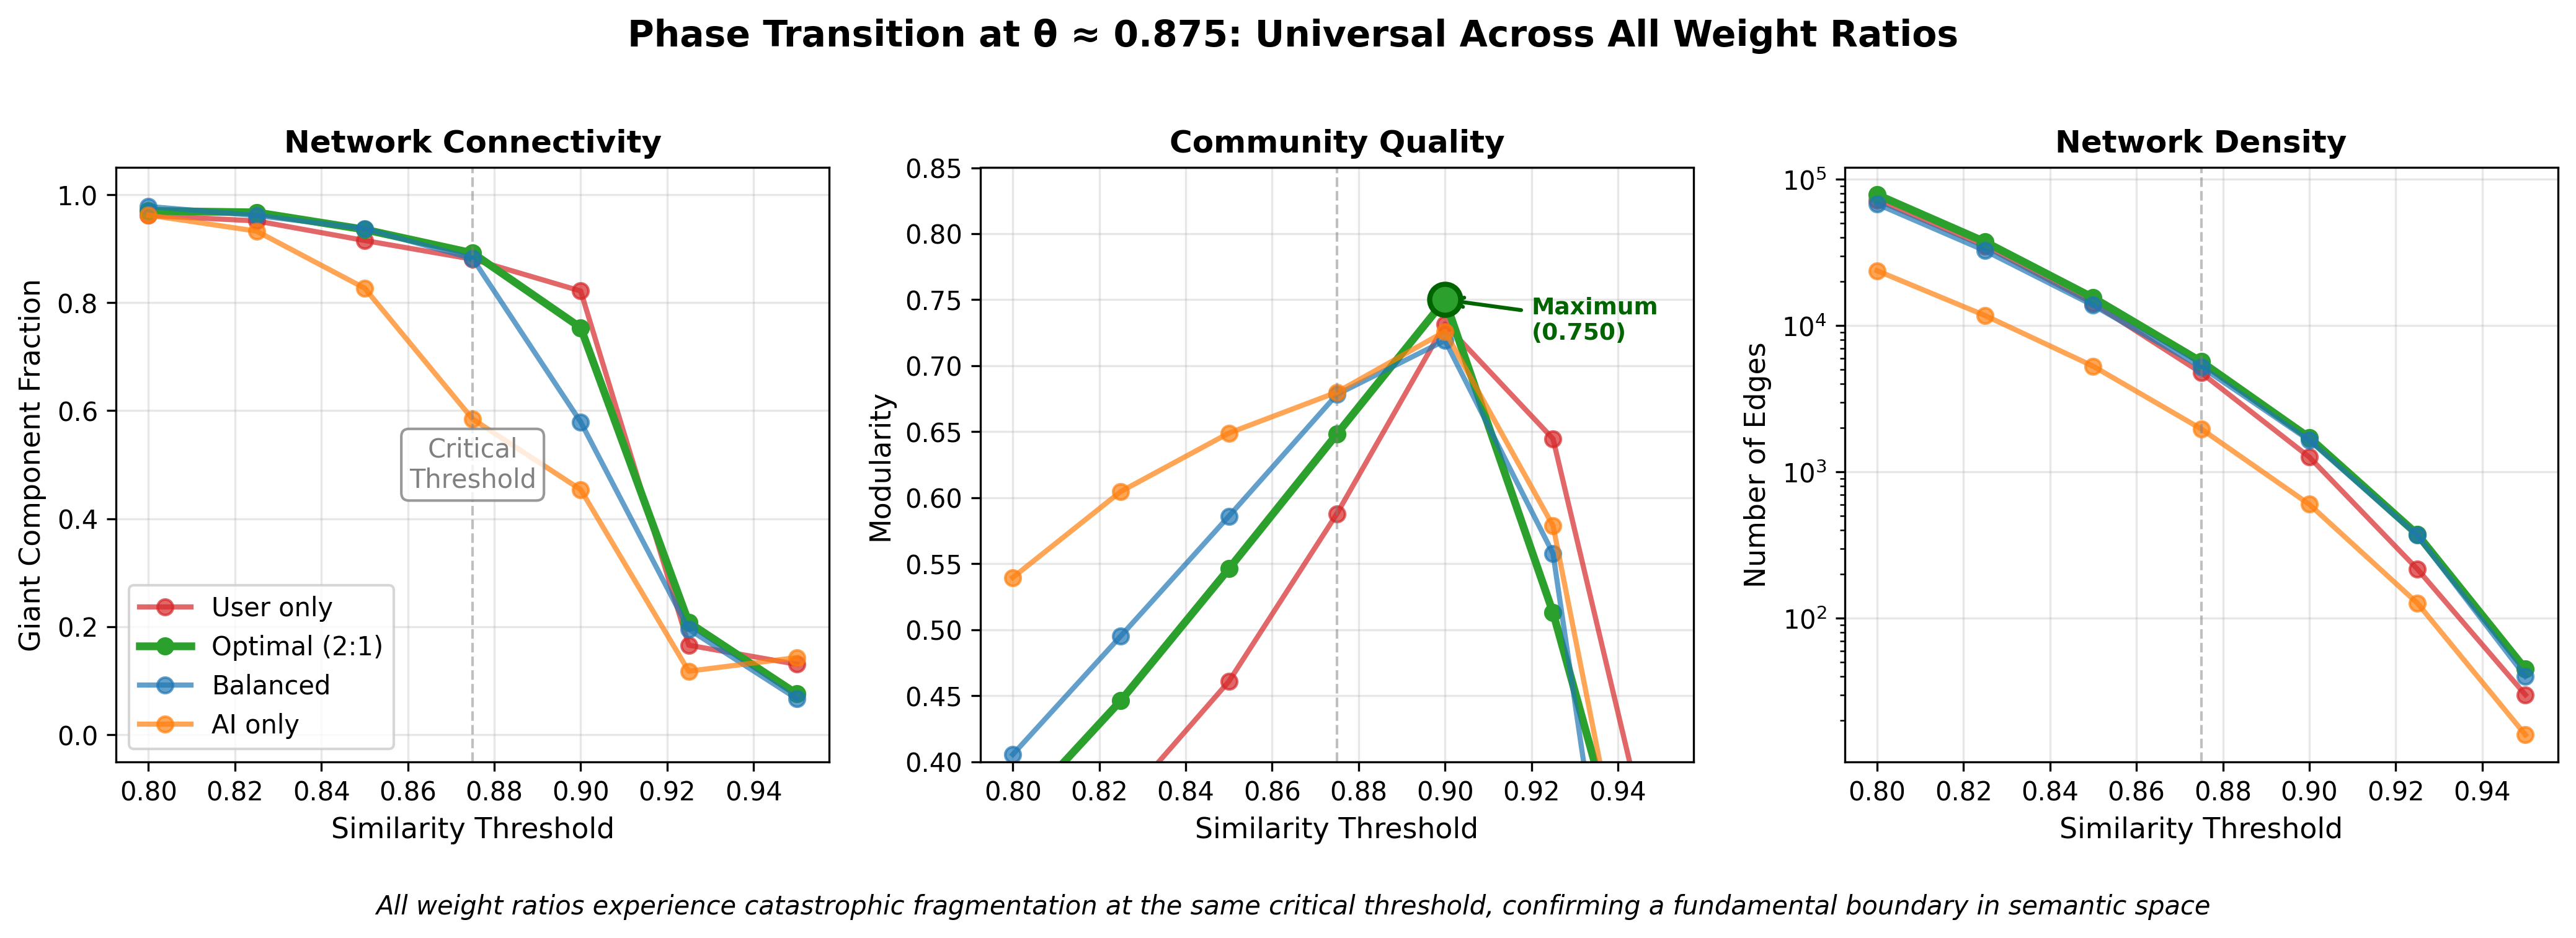
\includegraphics[width=\textwidth]{./images/threshold_evolution_clean.png}
\caption{Network metric evolution across similarity thresholds. All weight ratios experience catastrophic fragmentation at $\theta \approx 0.875$, indicating a universal percolation threshold in semantic space.}
\label{fig:phase_transition}
\end{figure}

Figure~\ref{fig:phase_transition} reveals a critical phase transition at similarity threshold $\theta \approx 0.875$. Below this threshold, the network maintains >90\% connectivity; above it, catastrophic fragmentation occurs. This percolation phenomenon is remarkably consistent across all weight ratios, suggesting a fundamental boundary in semantic coherence. Table~\ref{tab:threshold_comparison} provides detailed metrics comparing the network at our chosen 0.9 threshold versus 0.875, showing that lowering the threshold incorporates 376 additional nodes (83.7\% increase) and 4,037 edges (250\% increase), while network diameter and average path length decrease by 32\% and 33\% respectively.

\begin{table}[h]
\centering
\caption{Network Properties at Critical Thresholds (2:1 Weight Ratio)}
\label{tab:threshold_critical}
\begin{tabular}{lccccc}
\toprule
\textbf{Threshold} & \textbf{Nodes} & \textbf{Edges} & \textbf{Giant Comp.} & \textbf{Modularity} & \textbf{Communities} \\
\midrule
0.850 & 1,210 & 15,523 & 93.6\% & 0.546 & 13 \\
0.875 & 934 & 5,675 & 89.2\% & 0.648 & 15 \\
\textbf{0.900} & \textbf{601} & \textbf{1,718} & \textbf{75.4\%} & \textbf{0.750} & \textbf{15} \\
0.925 & 284 & 375 & 20.8\% & 0.513 & 5 \\
\bottomrule
\end{tabular}
\end{table}

\begin{table}[h]
\centering
\caption{Detailed Network Metrics Comparison at Different Similarity Thresholds}
\label{tab:threshold_comparison}
\begin{tabular}{l@{\hspace{1cm}}c@{\hspace{1cm}}c}
\toprule
\textbf{Metric} & \textbf{0.9 Threshold} & \textbf{0.875 Threshold} \\
\midrule
Number of Nodes & 449 & 825 \\
Edges & 1615 & 5652 \\
Average Degree & 7.19 & 13.7 \\
Network Diameter & 18 & 12 \\
Graph Density & 0.016 & 0.017 \\
Modularity & 0.75 & 0.65 \\
Avg. Clustering Coefficient & 0.6 & 0.6 \\
Avg. Path Length & 5.81 & 3.9 \\
\bottomrule
\end{tabular}
\end{table}

\subsubsection{Optimal Weight Ratio Determination}

\begin{figure}[h]
\centering
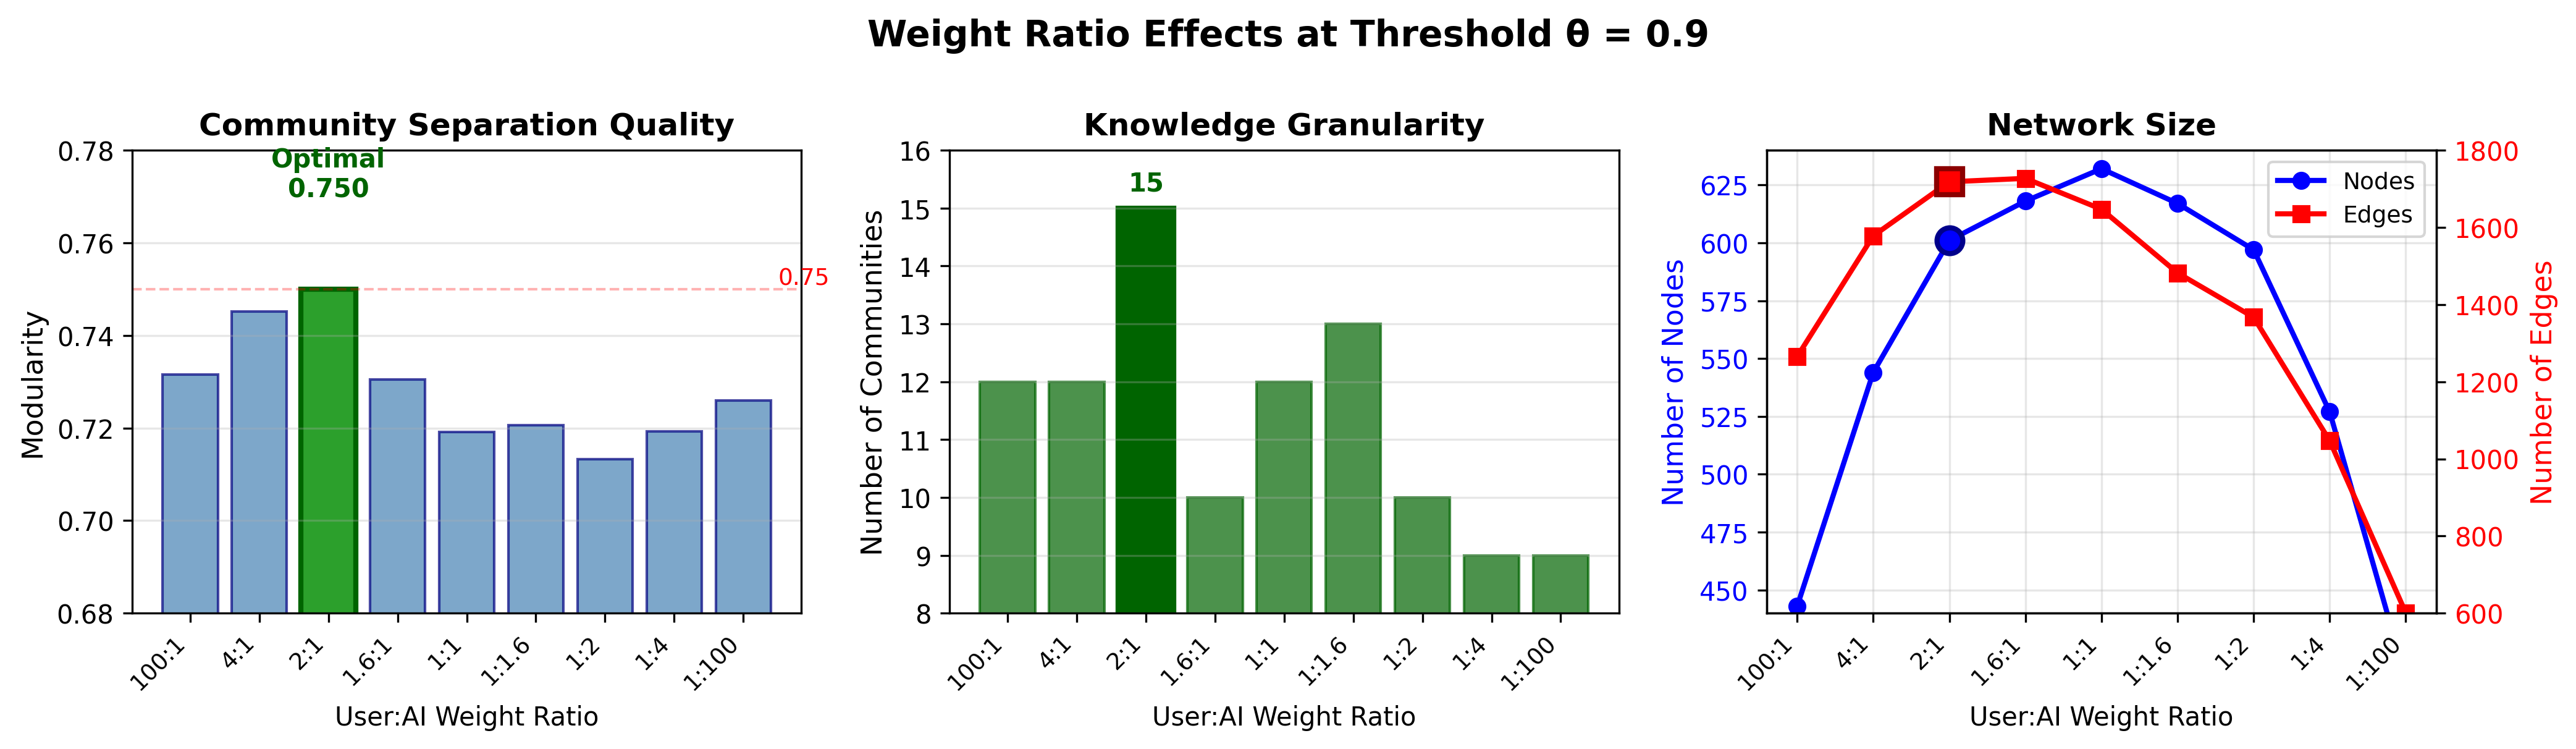
\includegraphics[width=\textwidth]{./images/weight_ratio_analysis_clean.png}
\caption{Weight ratio effects at threshold $\theta = 0.9$, showing three core metrics. The 2:1 user:AI ratio (green) achieves maximum modularity (0.750) with 15 distinct communities, providing optimal balance between community separation and network coherence.}
\label{fig:weight_ratio_analysis}
\end{figure}

At our chosen threshold of 0.9, systematic variation of weight ratios reveals that the 2:1 user:AI configuration maximizes modularity (0.750) while preserving network coherence. Figure~\ref{fig:weight_ratio_analysis} demonstrates how this ratio achieves optimal balance across multiple metrics.

\subsubsection{Knowledge Organization Across Weight Ratios}

Beyond quantitative metrics, weight ratios fundamentally alter how knowledge organizes into communities. Our analysis of topic distributions within detected communities reveals three distinct organizational regimes:

\begin{figure}[h]
\centering
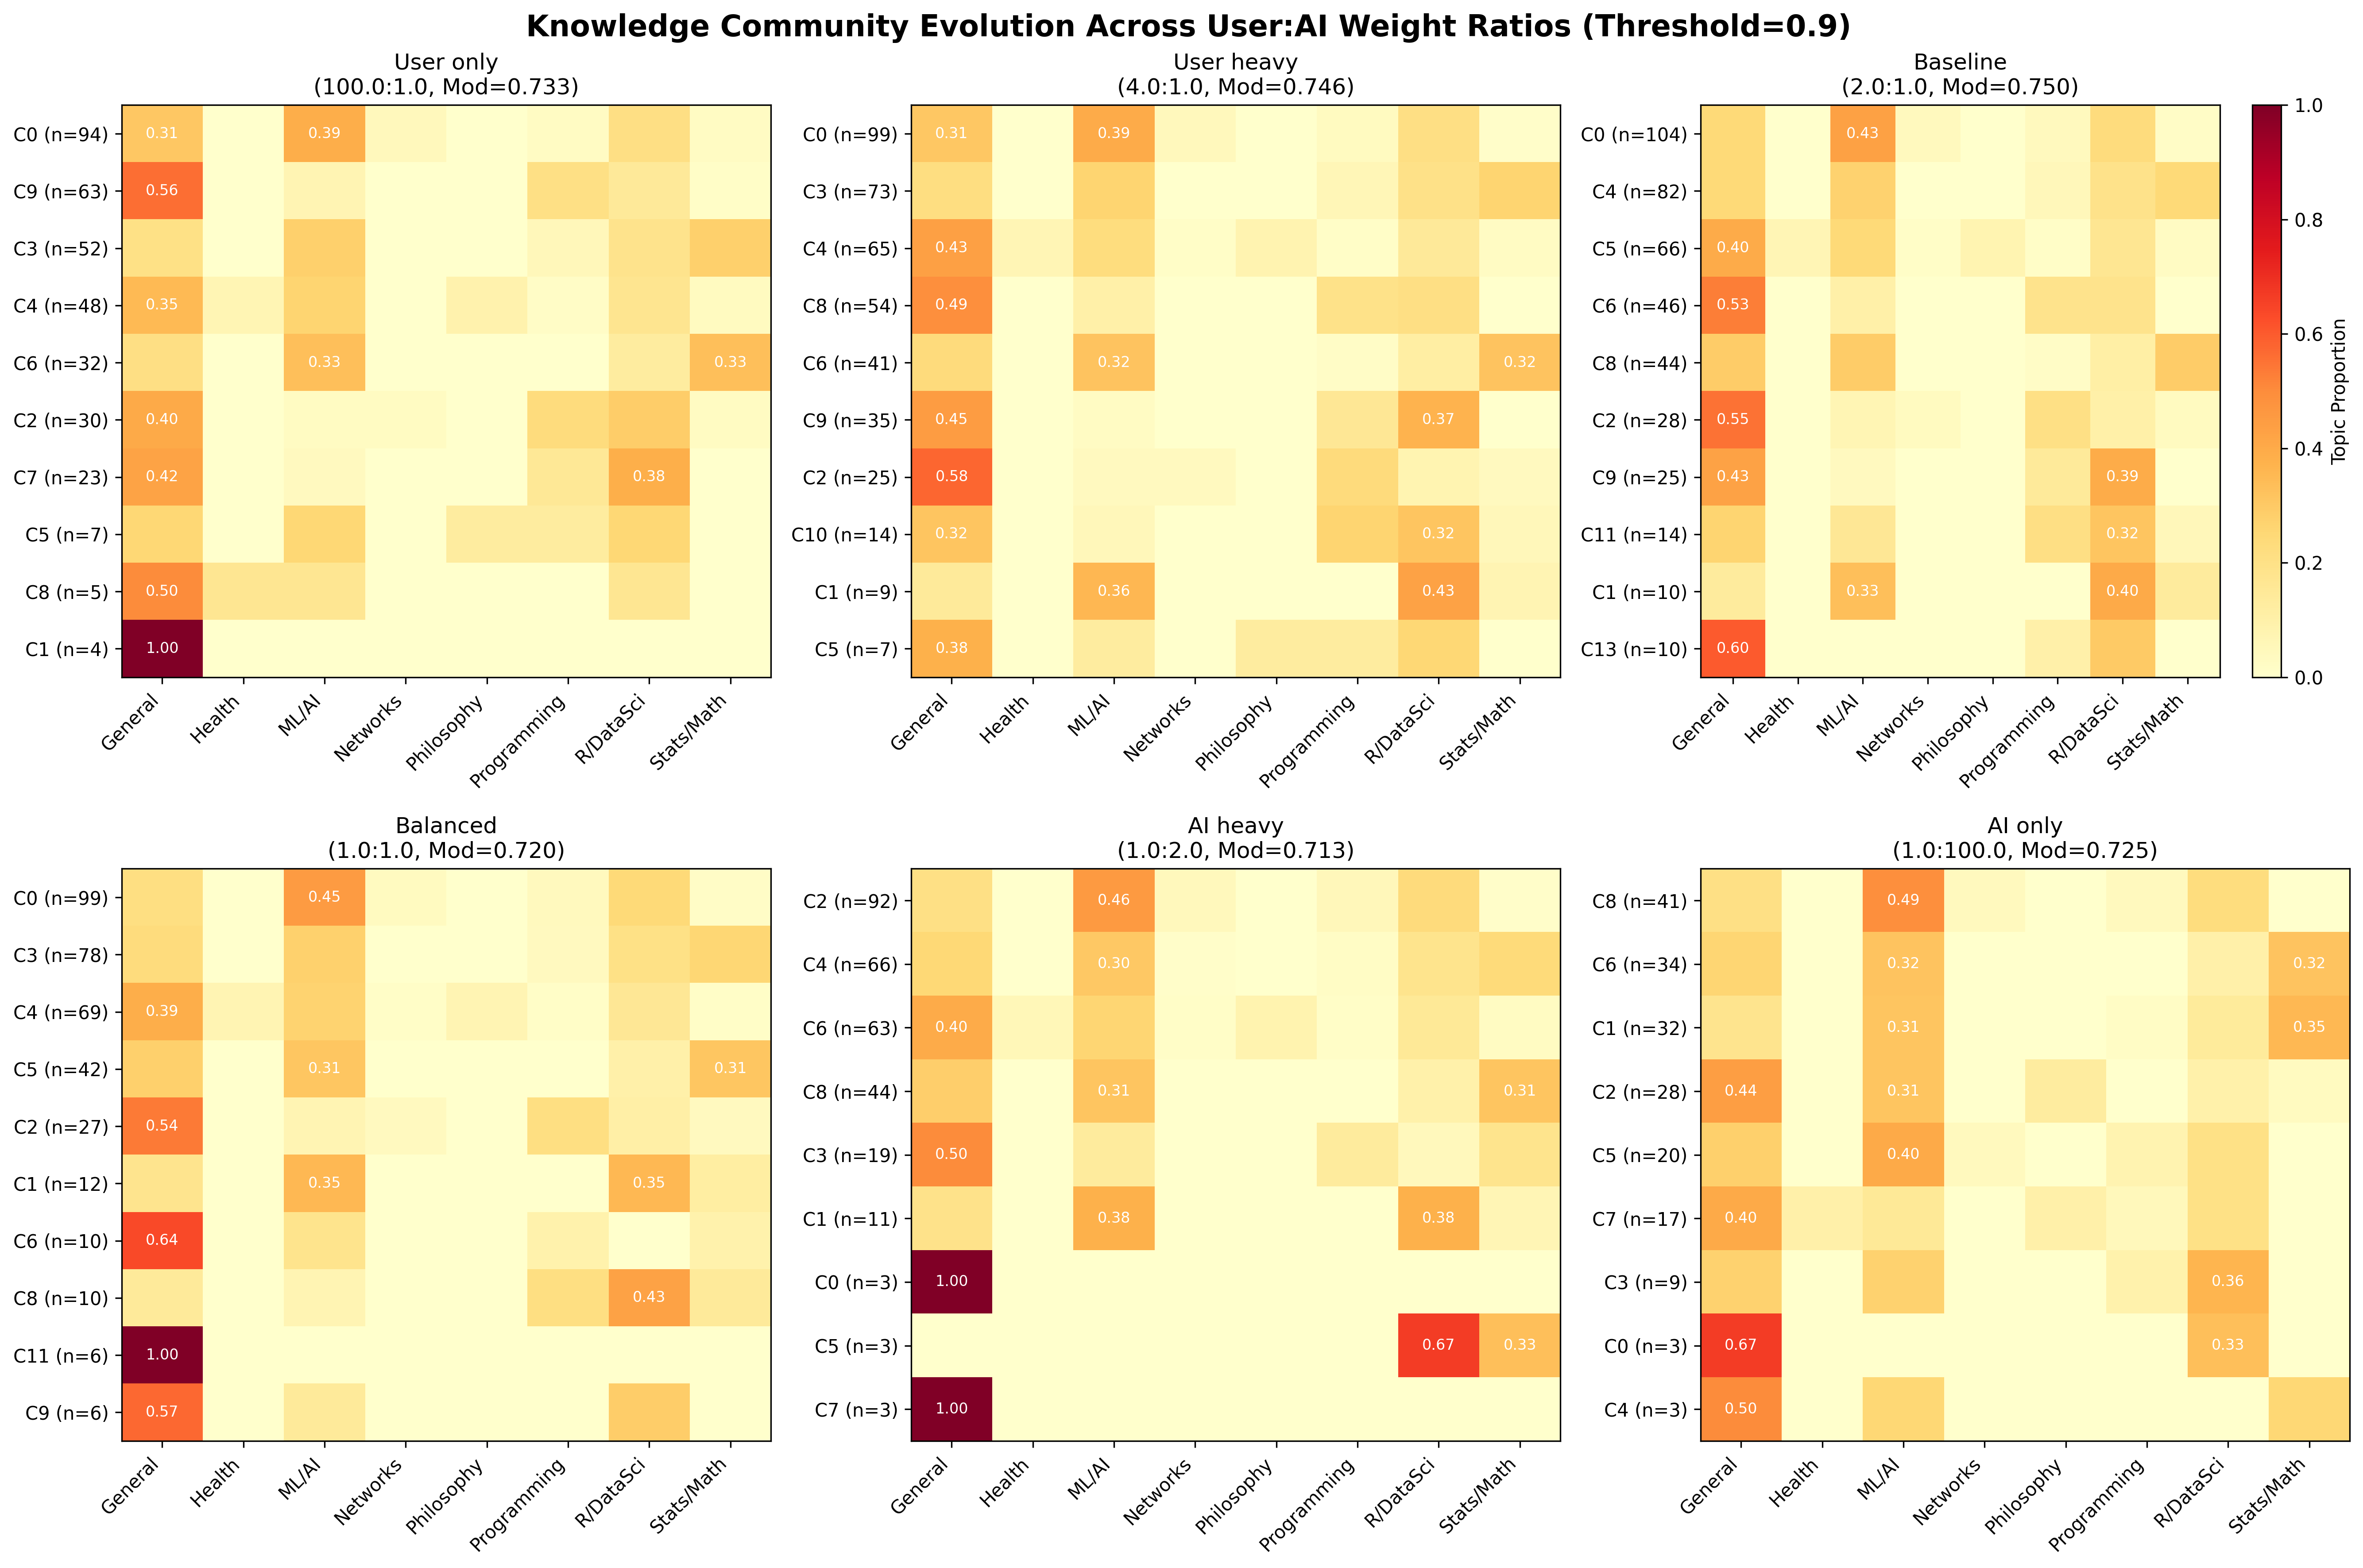
\includegraphics[width=\textwidth]{./images/community_topic_evolution.png}
\caption{Evolution of knowledge community structure across weight ratios at threshold 0.9. Heatmaps show topic proportion within each community, revealing transition from user-driven organization to AI response patterns.}
\label{fig:community_evolution}
\end{figure}

\textbf{User-Heavy Ratios (100:1, 4:1):} Communities reflect the user's mental organization with clear domain boundaries. ML/AI conversations remain distinct from Statistics discussions, which separate from Philosophy. Topic purity within communities exceeds 40\%, indicating focused knowledge domains.

\textbf{Balanced Ratio (2:1):} Our chosen configuration preserves topic focus while incorporating semantic breadth from AI responses. This produces 15 well-defined communities with the highest modularity (0.750). Each community maintains a dominant topic (30-45\% concentration) while including related subdisciplines that AI naturally connects.

\textbf{AI-Heavy Ratios (1:4, 1:100):} Communities reorganize around AI response patterns rather than knowledge domains. Technical topics merge based on how AI structures answers, reducing modularity and topic purity. The network reflects AI's knowledge organization rather than human cognitive structure.

\subsubsection{Case Study: Semantic Boundaries at the Phase Transition}

The phase transition at $\theta = 0.875$ reveals more than statistical fragmentation—it exposes semantic boundaries between distinct conversational contexts, as illustrated in Figure~\ref{fig:semantic_boundary}:

\begin{figure}[h]
\centering
\begin{subfigure}{0.48\textwidth}
    \centering
    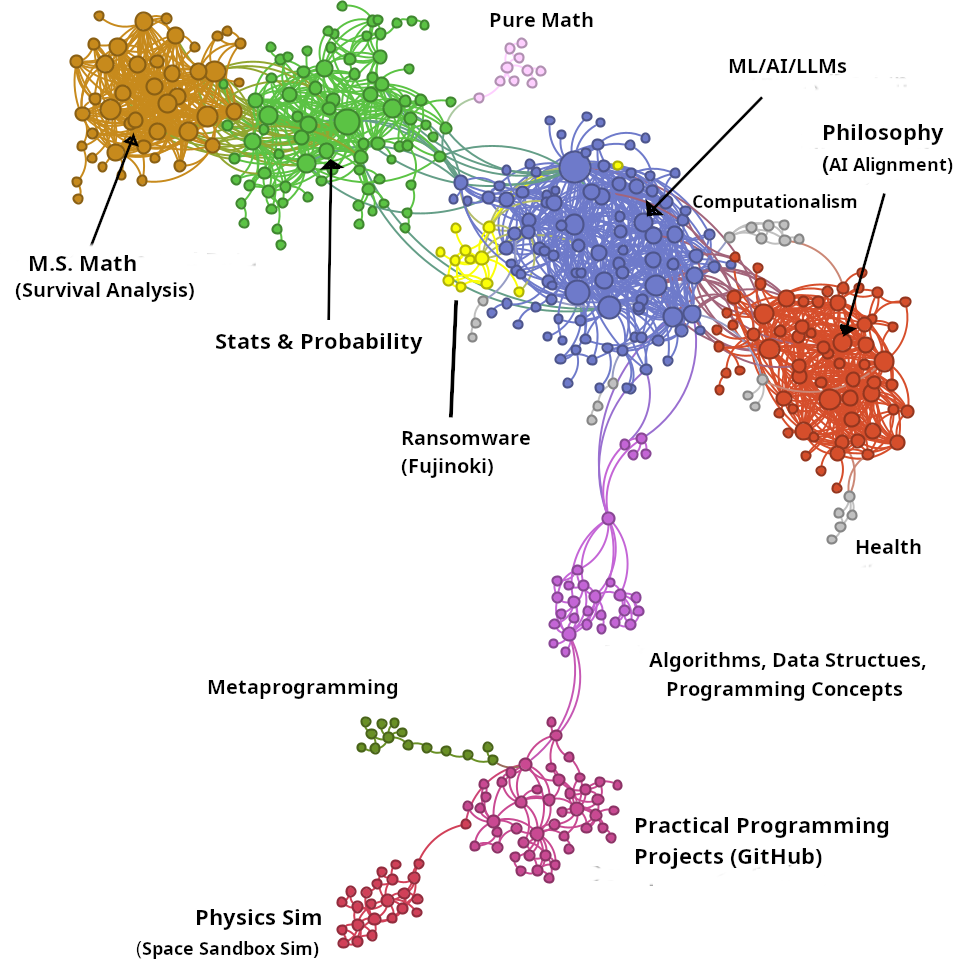
\includegraphics[width=\textwidth]{./images/cluster-vis-topics-better.png}
    \caption{$\theta=0.9$: Distinct contexts separated}
\end{subfigure}
\hfill
\begin{subfigure}{0.48\textwidth}
    \centering
    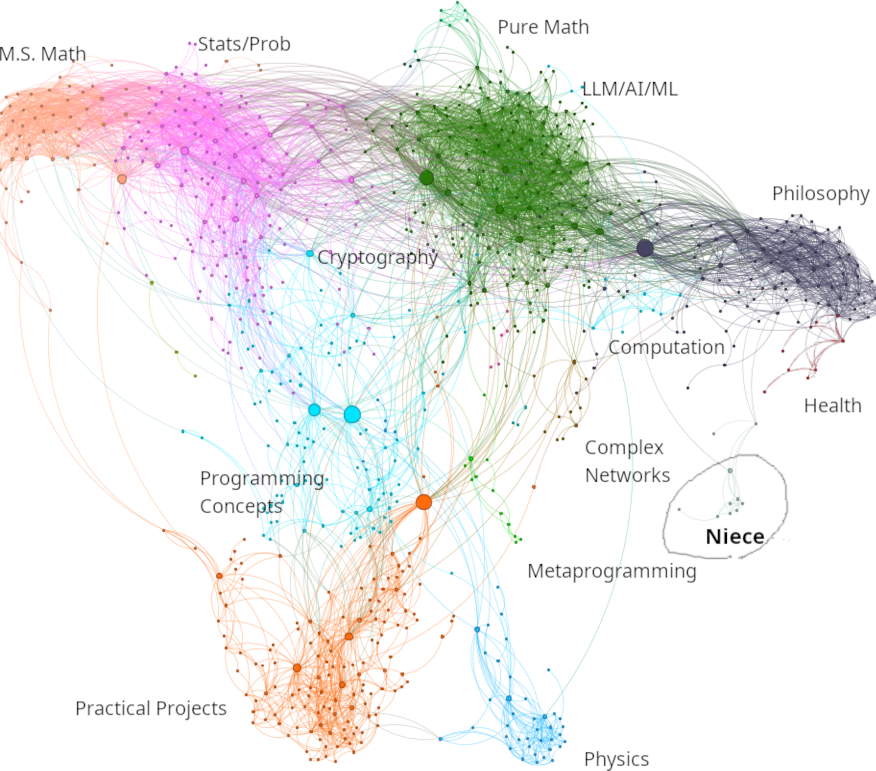
\includegraphics[width=\textwidth]{./images/0.875-wild-better.png}
    \caption{$\theta=0.875$: Peripheral context emerges}
\end{subfigure}
\caption{Semantic boundary crossing. At $\theta=0.9$, conversations with the author's niece remain isolated. At $\theta=0.875$, they connect through philosophical bridges, revealing 12.5\% semantic distance between conversational styles.}
\label{fig:semantic_boundary}
\end{figure}

As shown in Figure~\ref{fig:semantic_boundary}, conversations with the author's 13-year-old niece—characterized by artistic topics, informal language, and creative storytelling—remain isolated at threshold 0.9 (left panel) but connect to the giant component at 0.875 (right panel) through philosophical bridge conversations. This 2.5\% difference in similarity threshold captures the semantic distance between:

\begin{itemize}
    \item Primary knowledge network: Technical vocabulary, formal register, domain expertise
    \item Peripheral context: Age-appropriate explanations, creative topics, informal style
\end{itemize}

This validates our threshold selection: $\theta=0.9$ preserves analytical clarity by maintaining natural boundaries between cognitive contexts.

\subsubsection{Parameter Selection Justification}

Our comprehensive ablation study confirms the optimality of threshold 0.9 with 2:1 user:AI weighting:

\begin{enumerate}
    \item \textbf{Maximum modularity} (0.750) ensures clear community boundaries
    \item \textbf{Post-transition operation} removes noise while preserving essential connections (1,718 edges from 1.8M possible)
    \item \textbf{Semantic coherence} maintains topic-focused communities reflecting human knowledge organization
    \item \textbf{Boundary preservation} separates distinct conversational contexts while revealing their connection points
\end{enumerate}

\begin{table}[h]
\centering
\caption{2D Parameter Sweep Heatmap Summary}
\label{tab:2d_summary}
\begin{tabular}{lccccc}
\toprule
\textbf{Metric} & \textbf{Primary Driver} & \textbf{Secondary Effect} & \textbf{Optimal Config} \\
\midrule
Giant Component & Threshold & None & $\theta \leq 0.875$ \\
Modularity & Both & Weight ratio modulates & 2:1 at $\theta=0.9$ \\
Clustering & Weight ratio & Threshold modulates & User-heavy ratios \\
Density & Threshold & None & Application-dependent \\
Topic Coherence & Weight ratio & N/A & 2:1 to 4:1 \\
\bottomrule
\end{tabular}
\end{table}

The independence of threshold effects (controlling connectivity) from weight ratio effects (controlling organization) suggests these parameters tune orthogonal aspects of network structure. Threshold acts as a \emph{semantic filter} determining which connections exist, while weight ratio provides \emph{semantic perspective} determining how knowledge organizes within the connected structure.